\newpage
\section{Exercises: Arbitrary Frequency Response Filters}

\begin{marginfigure}
\begin{center}
    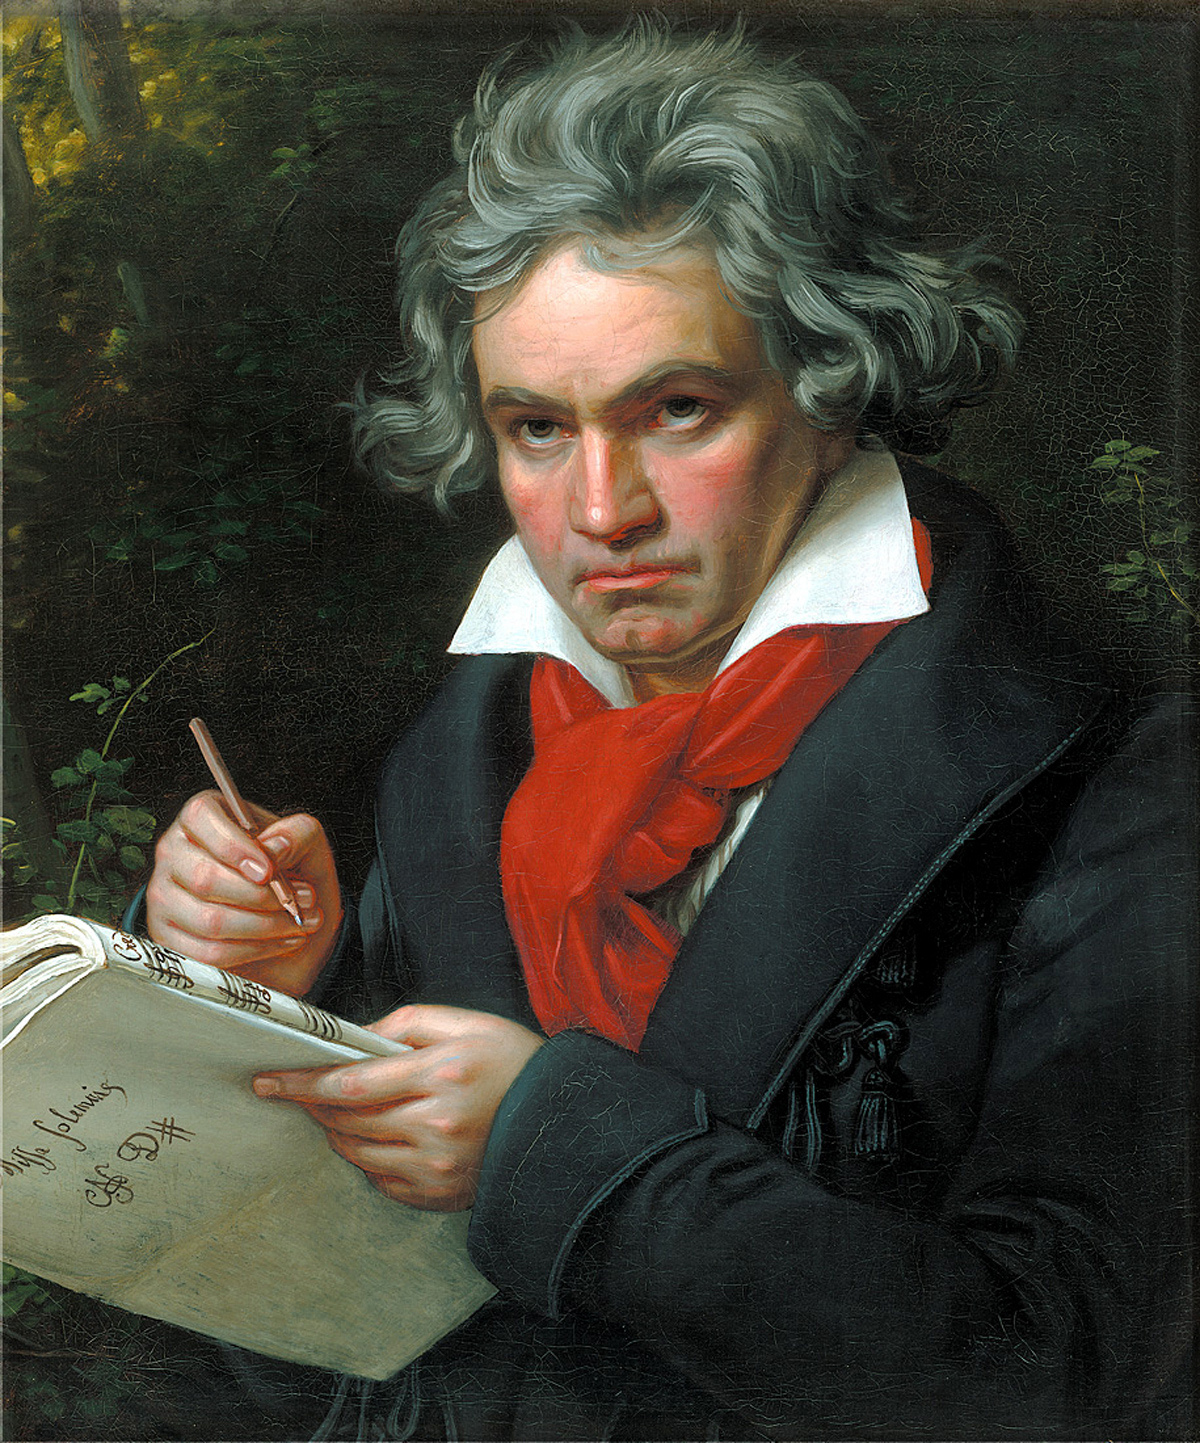
\includegraphics[height=0.25\textheight]{ch17/figures/Beethoven.jpg}
\end{center}
\caption{Ludwig van Beethoven, a well known musical composer active around the turn of the 18th and 19th century.}
\label{fig:beet}
\end{marginfigure}

\begin{enumerate}
\item The Python code in Listing \ref{lst:fftex} creates a signal consisting of narrowband sinusoids with large amplitudes ($x_1[n]$), and three time shifted unit impulses with weak amplitudes ($x_2[n]$):
  \begin{equation}
    x[n]=x_1[n]+x_2[n]
    \end{equation}

  \lstinputlisting[language=Python,caption={\texttt{fftex.py}},label=lst:fftex]{ch17/code/fftex.py}
  
  \begin{enumerate}[a)]
  \item Estimate the spectrum of the signal $x[n]$ using a Hann window $w[n]$ of length $N=16384$ to reduce spectral leakage.
    \begin{equation}
      \hat{x}_w[k]= \sum_{n=0}^{N-1}w[n]x[n]e^{-i\frac{2\pi}{N}nk}
      \end{equation}
      Use FFT to evaluate the DFT.

    Make a plot of the magnitude spectrum with power in dB scale
    $10\log_{10}|\hat{x}_w[\hat{\omega}_k]|^2$. Only plot the positive
    frequencies between 0 and $\pi$ with units of radians per
    sample. Identify the frequency ranges that are occupied by strong
    narrowband spectral components.
    
  \item Filter out the large magnitude frequency components in
    frequency domain and inverse DFT to obtain a time domain
    representation of the signal.
    \begin{equation}
    y[n]= \mathcal{F}_D^{-1}\left\{ \hat{h}[k]\hat{x}_w[k] \right\}
    \end{equation}
    Use FFT to evaluate the inverse DFT. Your plot should look like
    Figure \ref{fig:filtered_weak_signal}.
    
    \item Explain why the filtered signal $y[n]$ still looks like the
      original weak signal $x_2[n]$ consisting of unit impulses, even
      though it is missing some frequency components.
    \end{enumerate}
    
\item
  

This task is a programming assignment. Your task will be to analyze
the time-frequency contents of a musical recording. The aim is to
determine what sequence of musical notes are being played. 

Download the audio file from:
\begin{center}
\verb|https://bit.ly/3EAhn26| 
\end{center}
You can listen to the audio file to get an idea of the time-frequency
contents of the signal.

Read the audio signal using Python as follows:
\begin{verbatim}
import scipy.io.wavfile
audio = scipy.io.wavfile.read("b.wav")
sample_rate=audio[0]
# read only one channel of the stereo signal
signal=audio[1][:,0]
\end{verbatim}

Complete the following tasks and justify your result:
\begin{enumerate}[a)]

\item What is the sample-rate? What is the lowest and highest
  frequency spectral component that can be represented using this
  sample-rate? 

\item Make a plot of the signal as a function of time. Use time in
  seconds on the horizontal axis. How long is the signal?
    
\item Write a short program to analyze the time-frequency contents of
  this signal. There are several Python library functions for
  implementing a spectrogram. For example:
  \verb|scipy.signal.spectrogram| or
  \verb|matplotlib.pyplot.specgram|. For this exercise, I ask that you
  do not use these functions, but implement your own function instead,
  so that you can gain a good understanding of how these functions are
  implemented. You can use the example program in Listing
  \ref{lst:dynamic_spectrum} to help you out. Use a Hann window in the
  spectral analysis.

\item Make a plot of the spectrogram produced with your program. Limit
  the frequency axis to range 0 to 1500 Hz. Use an appropriate time
  and frequency resolution that allows you to identify the positions
  of individual notes being played in time and frequency.

\item In the time-frequency spectrum of the musical instrument playing
  an individual note, there are spectral lines with multiple harmonics
  $f = n f_0$, where $n \in \mathbb{N}$ is a positive integer, and
  $f_0$ is the base frequency. For example, if $f_0= 220$ Hz, you will
  also see spectral lines at 440, 660, 880, and 1100 Hz. Why are there
  multiple spectral lines?

\item Using the spectrogram plot, determine what are the nine musical
  notes that are played in the recording? Make sure that your plot
  allows you to clearly identify each note in time and frequency. Use
  150 to 400 Hz on the frequency axis as the axis limits. You will
  most likely need to adjust the FFT length, overlap, and zero padding
  settings to be able to easily determine the notes. You might also
  need to adjust the color scale. I'll give you a hint. The first note
  is E.

Assume an equal tempered scale is used, which results in the following mapping of base frequencies and musical notes: 
\begin{center}
\begin{tabular}{c|c}
Note & Frequency (Hz) \\
\hline 
A & 220.0\\
A\# & 233.0819 \\
B & 246.9417 \\
C & 261.6256 \\
C\# & 277.1826 \\
D & 293.6648 \\
D\# & 311.127 \\
E & 329.6276 \\
F & 349.2282 \\
F\# & 369.9944 \\
G & 391.9954 
\end{tabular}
\end{center}




\end{enumerate}
\end{enumerate}
